\section{Specific requirements}

\subsection{External Interface Requirements}
In this section are described details about user interfaces, hardware and application programming interfaces.

\subsubsection{User Interfaces}
\begin{figure}[H]
    \subfloat[Details]{
        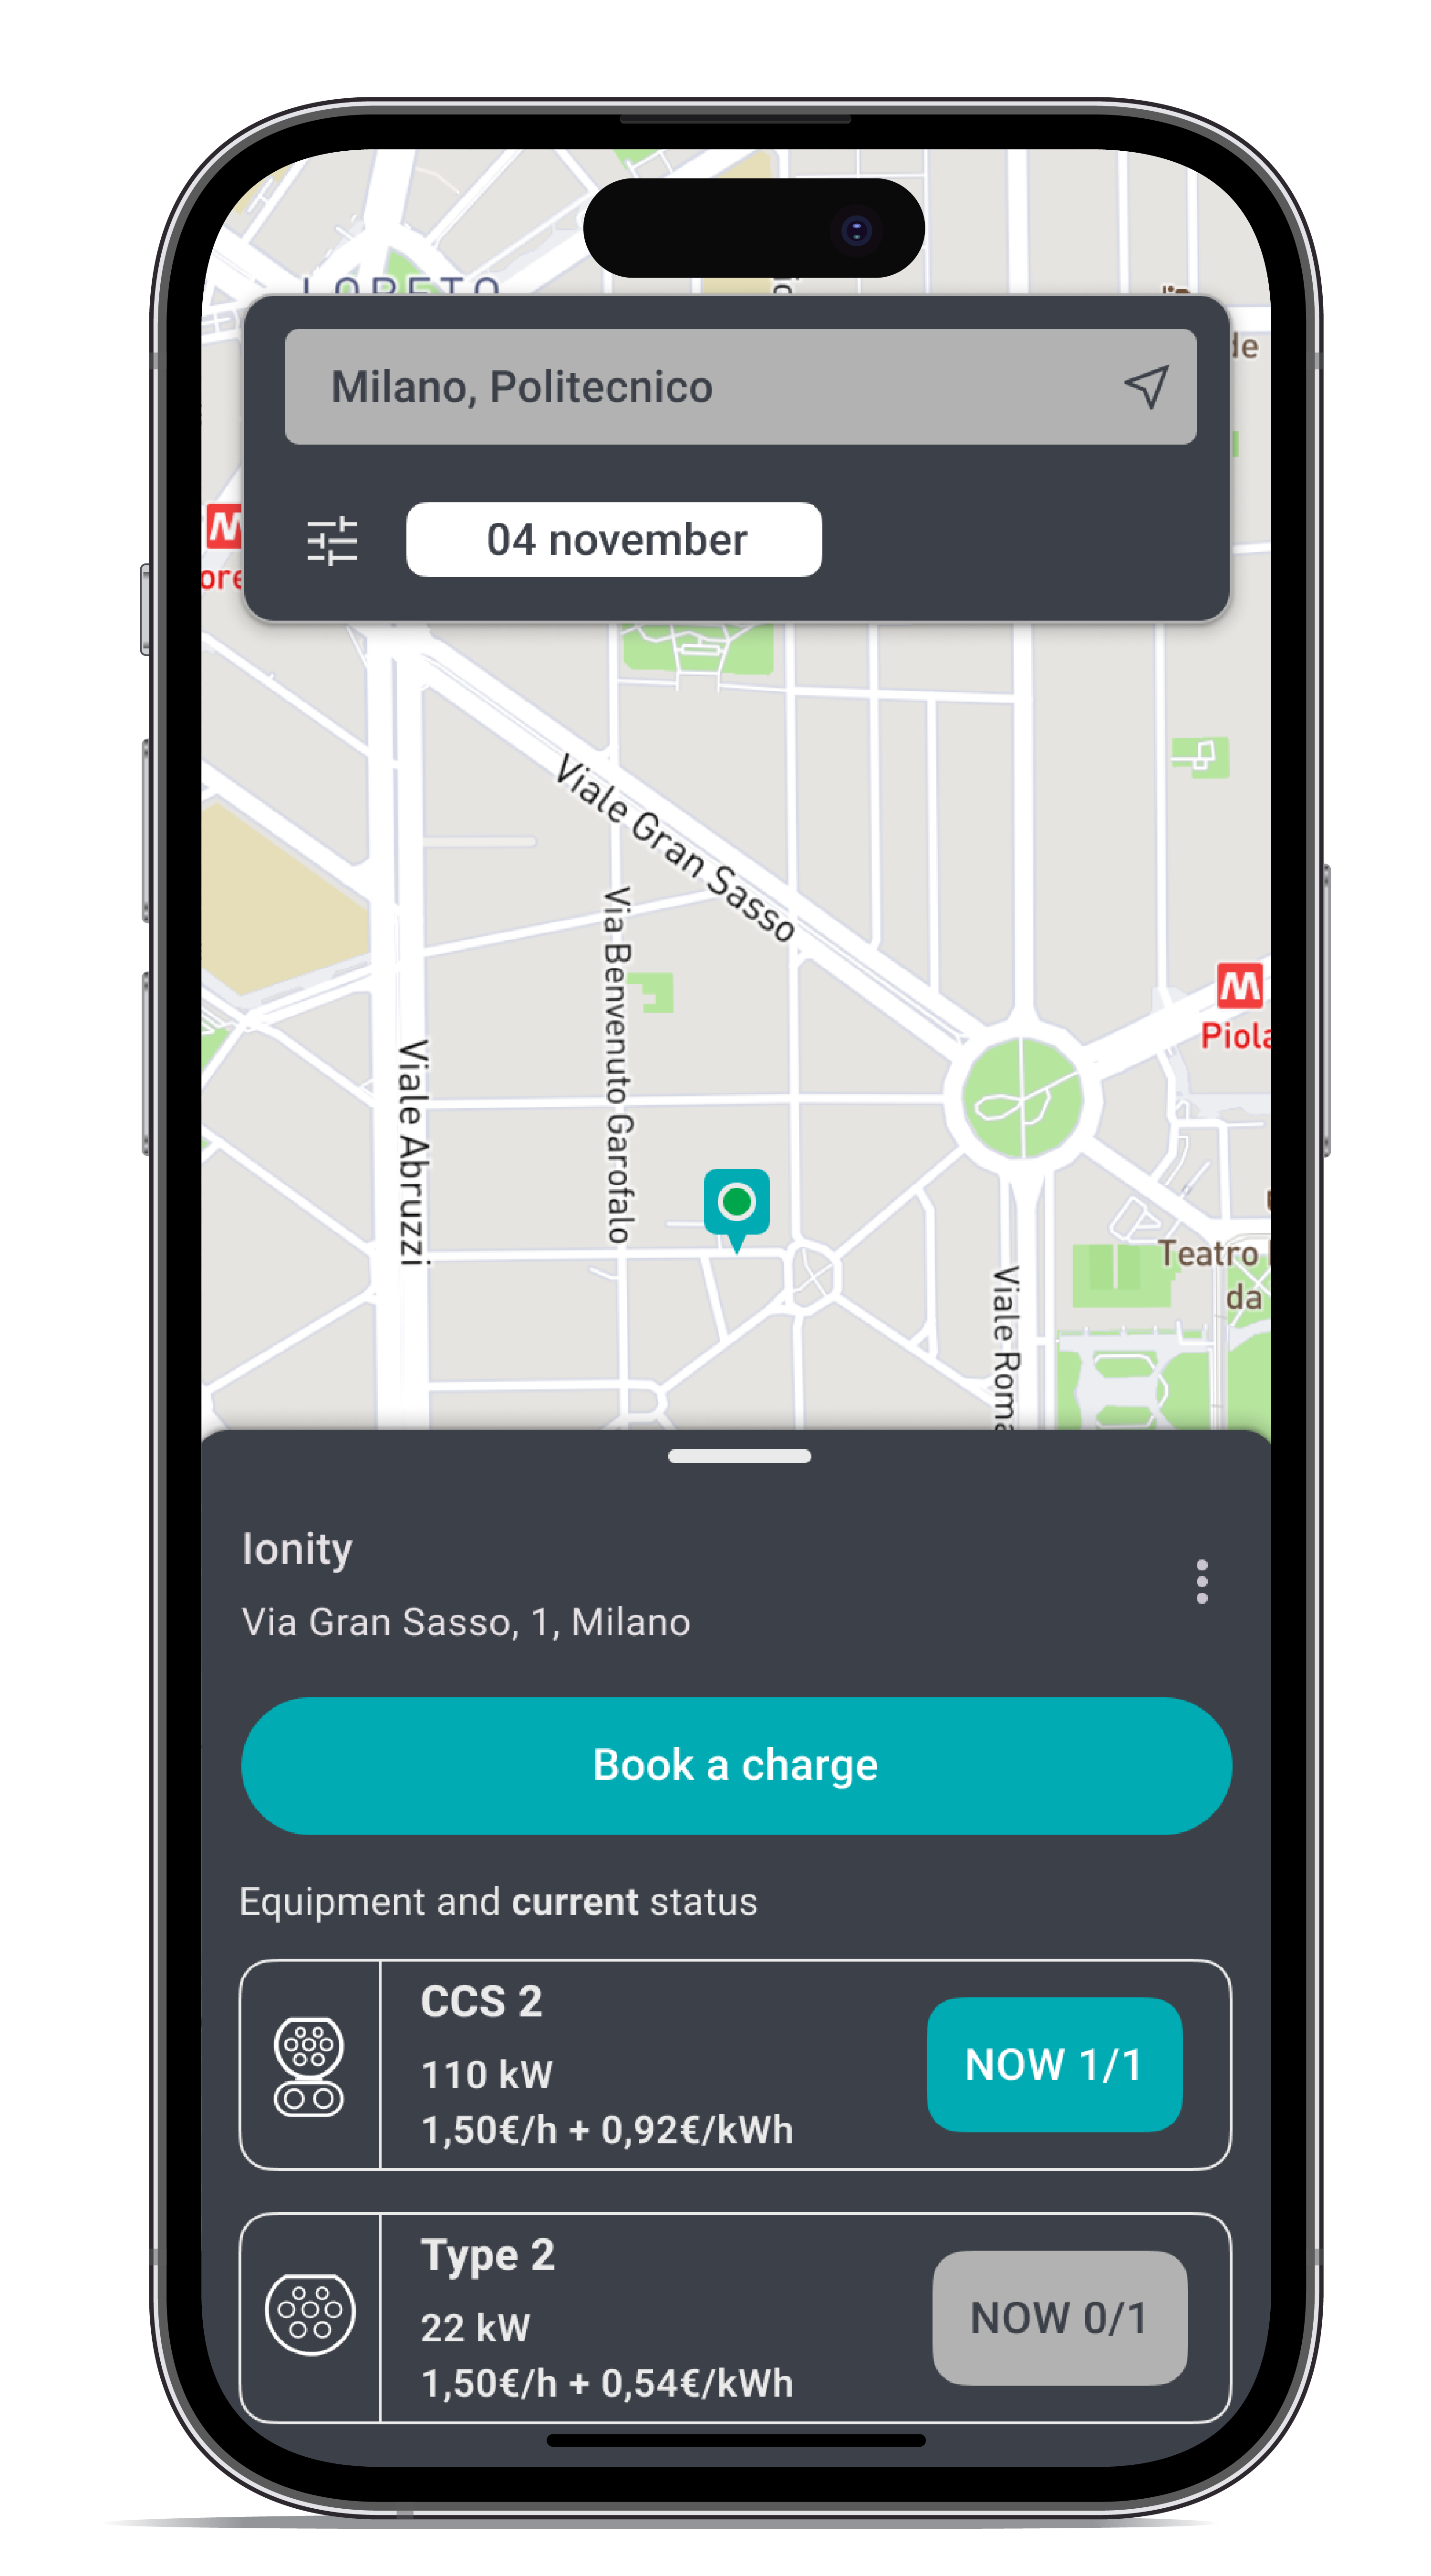
\includegraphics[scale=0.1]{src/mockups/details.png}
    }
    \subfloat[Booking]{
        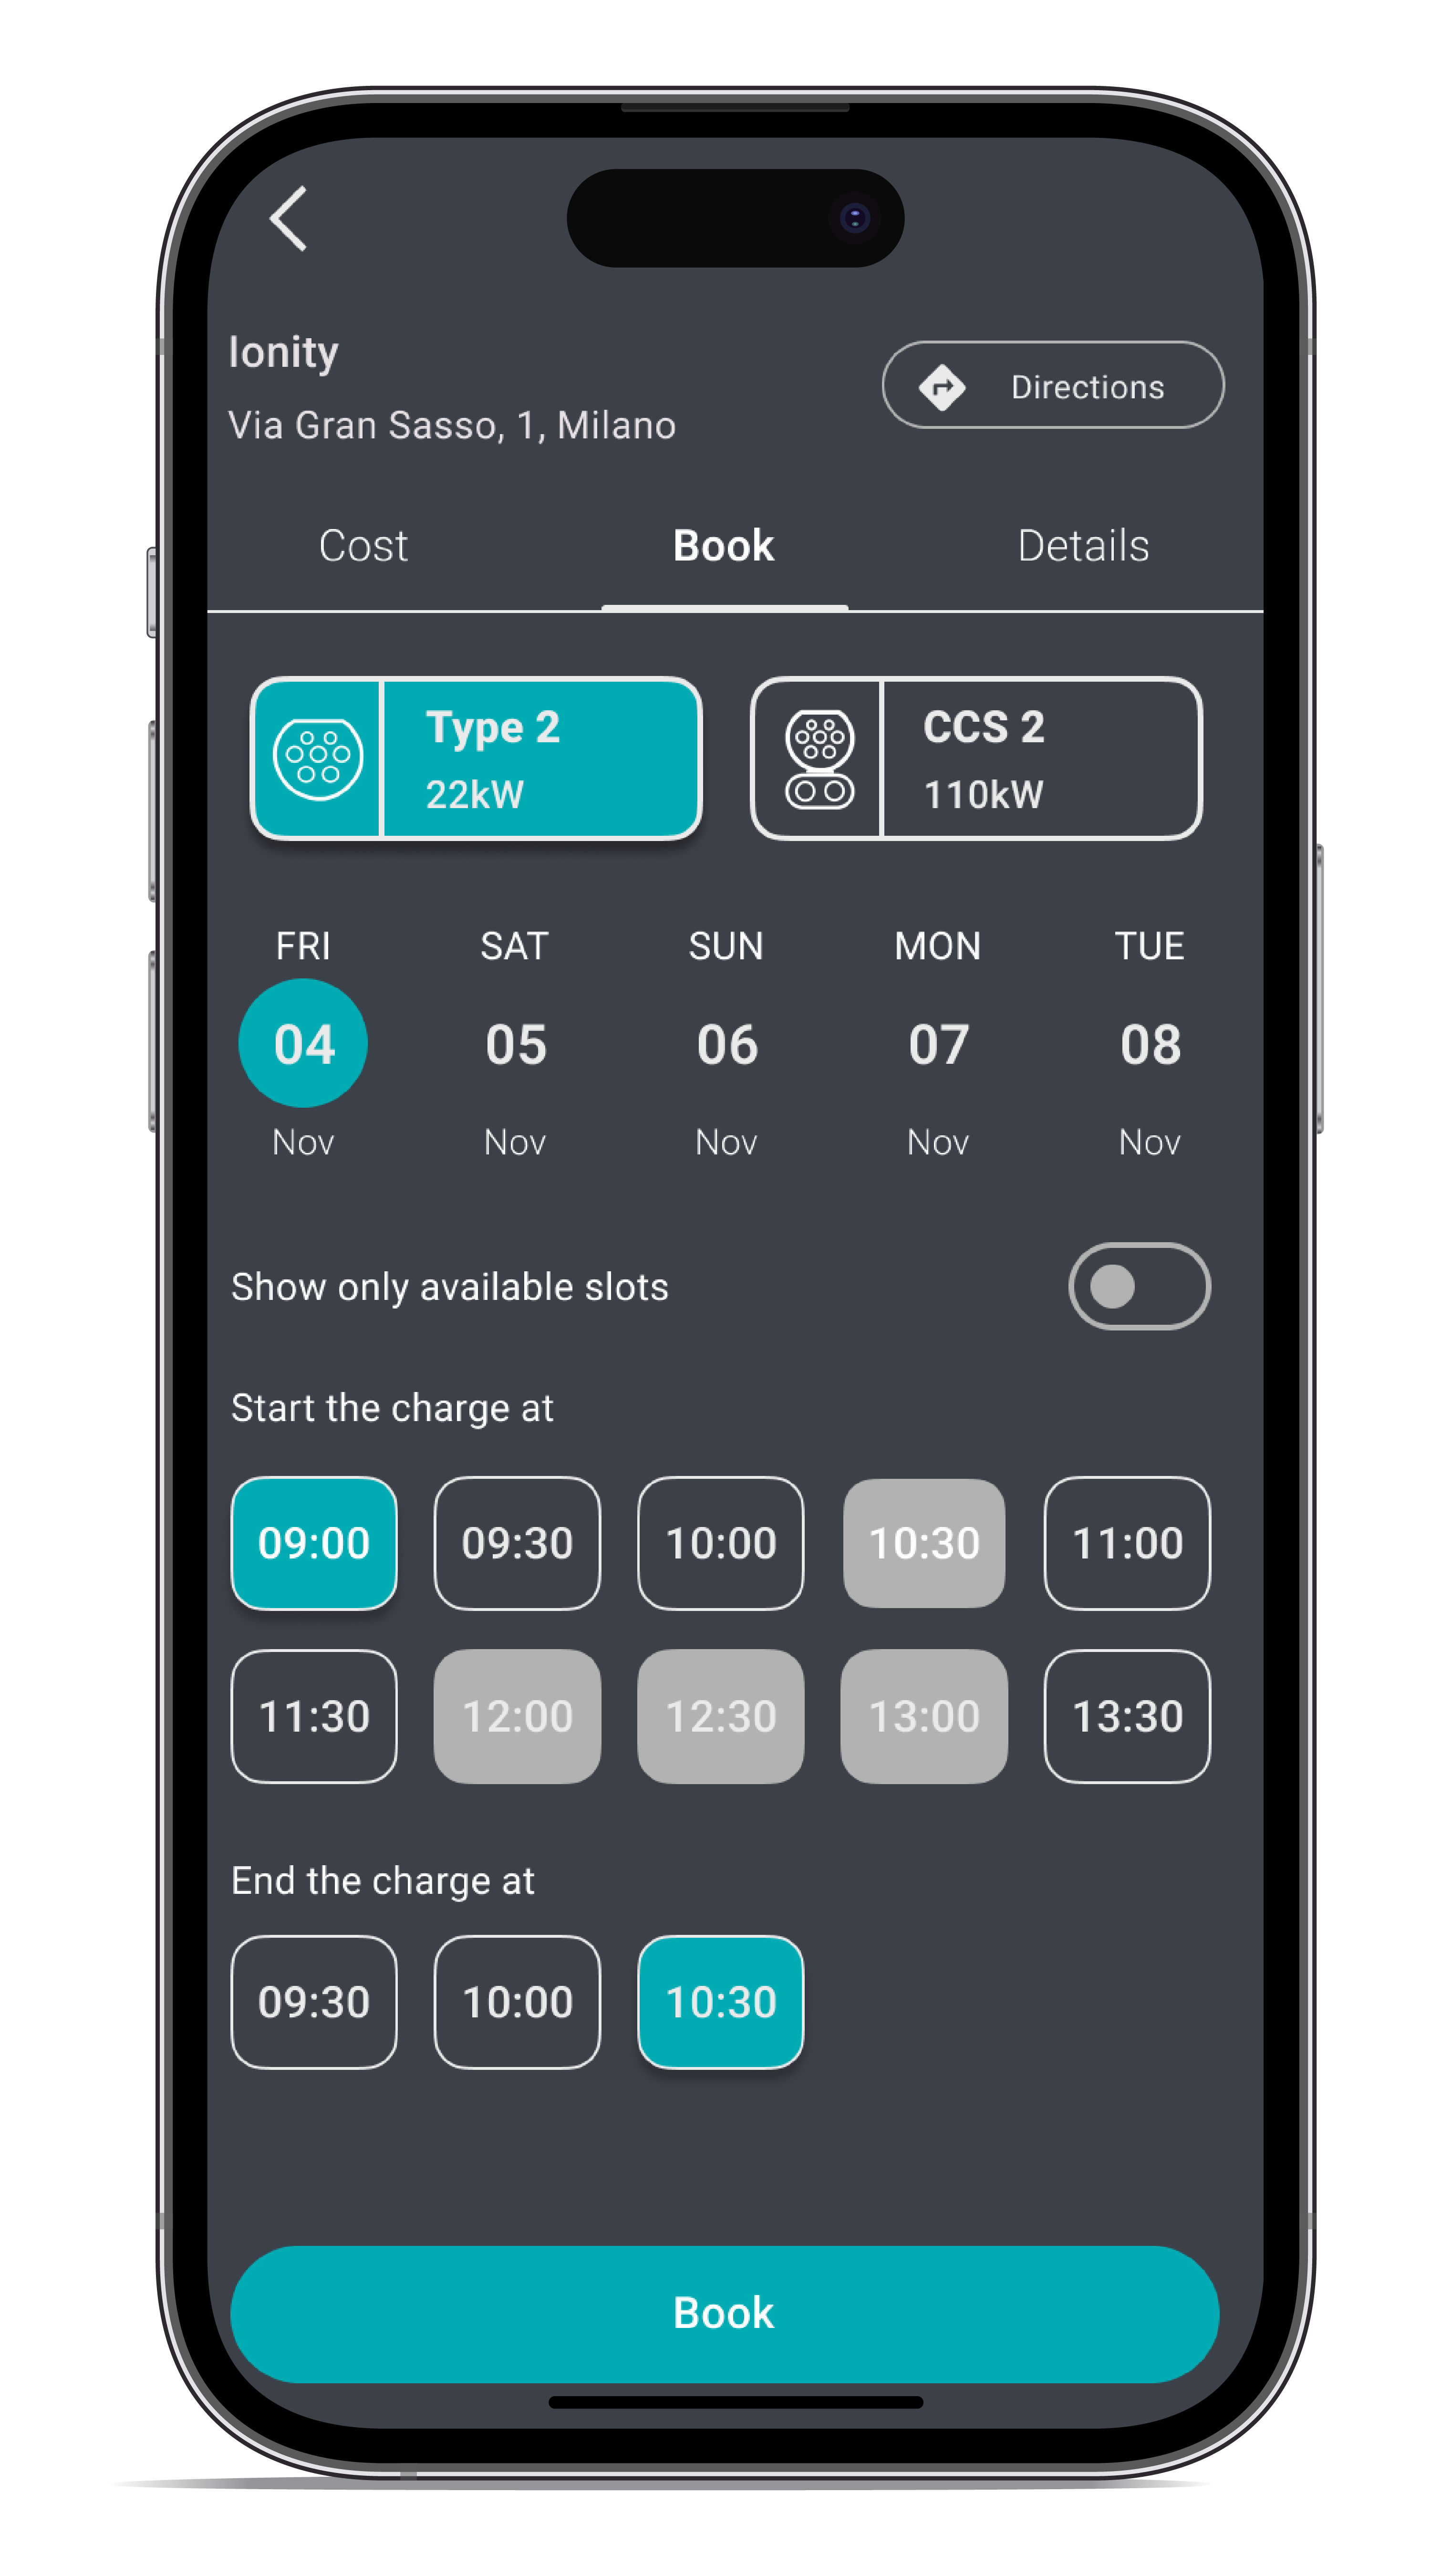
\includegraphics[scale=0.1]{src/mockups/book.png}
    }
    \subfloat[Cost detail]{
        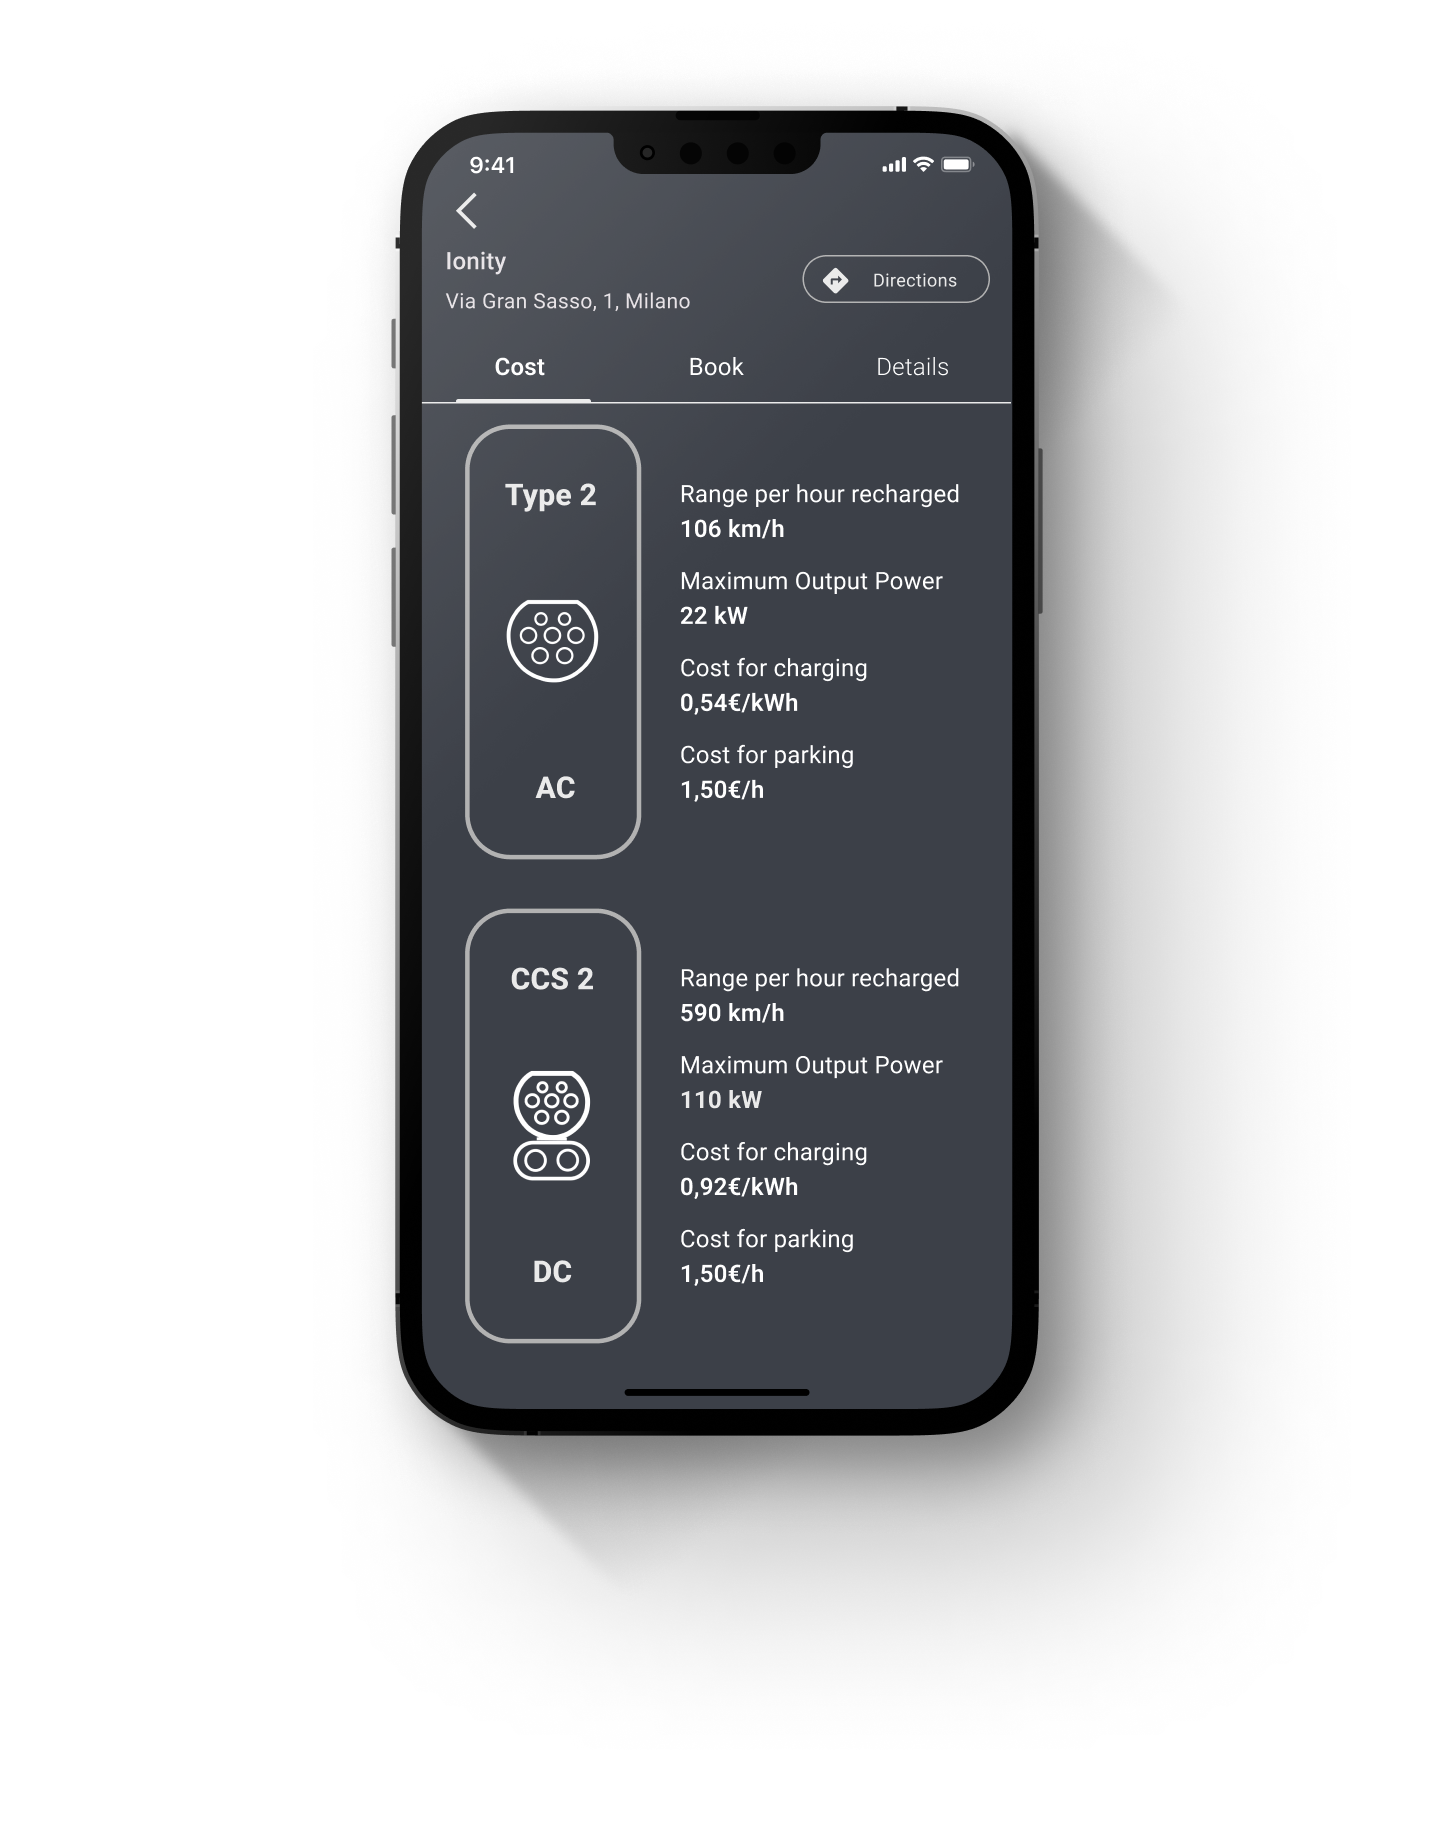
\includegraphics[scale=0.1]{src/mockups/book_cost.png}
    }
    \newline
    % following mockups
\end{figure}


\subsubsection{Hardware Interfaces}
Nothing here

\subsubsection{Software Interfaces}
Nothing here

\subsubsection{Communication Interfaces}
Nothing here

\subsection{Use cases}

\begin{figure}[H]
    \centering
    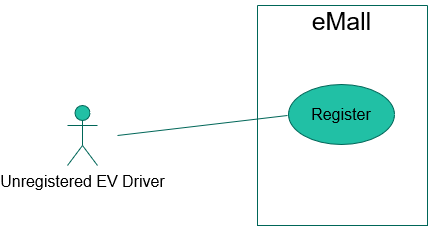
\includegraphics[scale=0.6]{src/use_case_diagram/driver_registration.png}
\end{figure}

\begin{figure}[H]
    \centering
    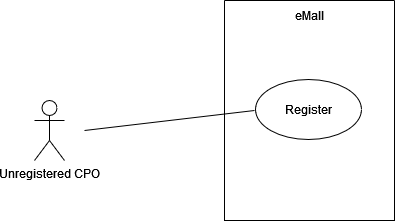
\includegraphics[scale=0.6]{src/use_case_diagram/cpo_registration.png}
\end{figure}

\begin{figure}[H]
    \centering
    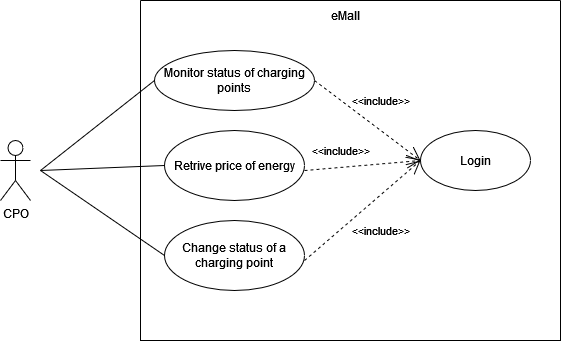
\includegraphics[scale=0.5]{src/use_case_diagram/cpo.png}
\end{figure}

\begin{figure}[H]
    \centering
    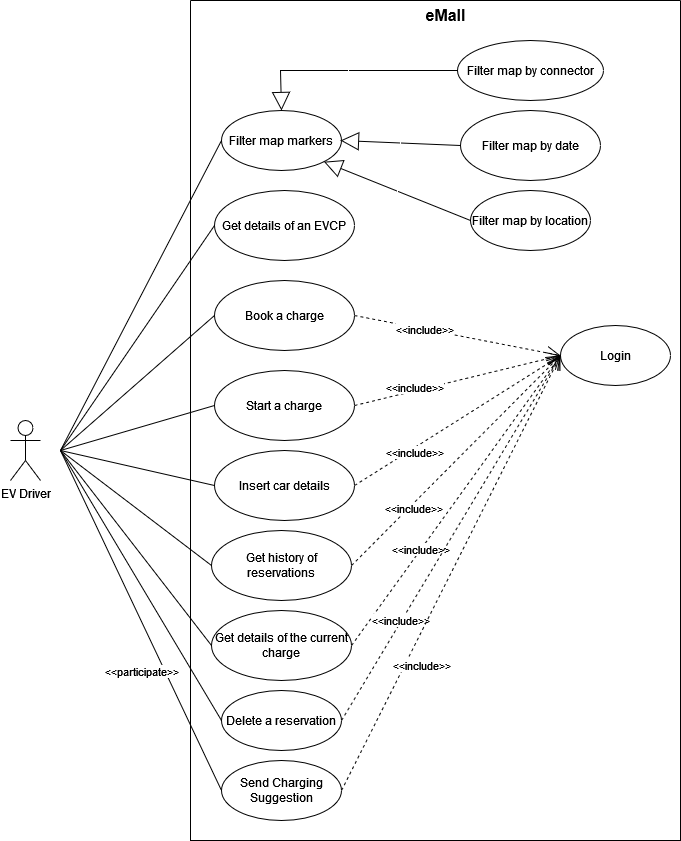
\includegraphics[scale=0.6]{src/use_case_diagram/driver.png}
\end{figure}

\usecase
{EV driver registration}
{EV driver}
{EV driver clicks 'Sign Up' in the application homepage}
{
    \begin{enumerate}
        \item The system sends user the registration form
        \item Driver enters name, surname, birth date, telephone number and password. Then submits the data upon reading and accepting the Privacy Policy and the Terms of Service
        \item The system sends a SMS to driver through an API containing a secret code
        \item The driver submits the received verification code
        \item The system verifies the code and displays a success message
    \end{enumerate}
}
{A new EV driver account is created}
{
    \begin{itemize}
        \item A required registration field is missing when the form is submitted
        \item A wrong verification code is submitted
        \item The timeout of verification expires
    \end{itemize}
}
{
    All the exception are treated the same: the system will notify user with a human-readable message and the user is redirected to the homepage
}

\usecase
{CPO registration} % name
{CPO} % actor
{CPO clicks 'Sign Up' in the business dedicated application homepage} % entry condition
{ % event flow
    \begin{enumerate}
        \item The system sends operator the registration form
        \item Operator enters company name, VAT, IBAN, and password. Then submits the data upon reading and accepting the Privacy Policy and the Terms of Service
        \item The system processes the provided information and display a success message
    \end{enumerate}
}
{A new operator account is created} % exit condition
{ % exceptions
    \begin{itemize}
        \item A required registration field is missing when the form is submitted
        \item The operator is not associated to the given VAT
    \end{itemize}
}
{ % notes
    All the exception are treated the same: the system will notify operator with a human-readable message and the operator is redirected to the homepage
}

\usecase
{Check energy in batteries} % name
{CPO} % actor
{Authenticated CPO is in "Monitor status of EVCP" tab} % entry condition
{ % event flow
    \begin{enumerate}
        \item The operator choose a specific EVCP and clicks 'check energy in batteries'
        \item The system shows the battery status of the selected EVCP, if any
    \end{enumerate}
}
{The 'Check energy in batteries' chart is shown} % exit condition
{ % exceptions
    \begin{itemize}
        \item ...
    \end{itemize}
}
{ % notes
    ...
}

\usecase
{Monitor specific charging process} % name
{CPO} % actor
{Authenticated CPO is in "Monitor status of CP" tab} % entry condition
{ % event flow
    \begin{enumerate}
        \item The operator choose a specific EVCP and clicks "monitor specific charging process"
        \item The system shows a list of active charging process and ask operator to choose one
        \item The operator choose a specific active charging process from the list
        \item The system shows the details of the chosen charging process
    \end{enumerate}
}
{The details of the specific charging process are displayed} % exit condition
{ % exceptions
    \begin{itemize}
        \item ...
    \end{itemize}
}
{ % notes
...
}

\usecase
{Monitor aggregate charging process} % name
{CPO} % actor
{Authenticated CPO is in "Monitor status of CP" tab} % entry condition
{ % event flow
    \begin{enumerate}
        \item The operator choose a specific EVCP and clicks "monitor aggregate charging process"
        \item The system shows a chart with a detailed view of aggregate charging processes
    \end{enumerate}
}
{The aggregate charging process details charts are displayed} % exit condition
{ % exceptions
    \begin{itemize}
        \item ...
    \end{itemize}
}
{ % notes
...
}

\usecase
{View historical reservations} % name
{CPO} % actor
{Authenticated CPO is in "View reservations" tab} % entry condition
{ % event flow
    \begin{enumerate}
        \item The operator choose a specific EVCP, choose "historical reservation" tab, and sets a specific time frame
        \item The system shows the reservation details of the chosen EVCP during the chosen time frame
    \end{enumerate}
}
{The details of the historical reservations are displayed} % exit condition
{ % exceptions
    \begin{itemize}
        \item ...
    \end{itemize}
}
{ % notes
...
}

\usecase
{View active reservations} % name
{CPO} % actor
{Authenticated CPO is in "View reservations" tab} % entry condition
{ % event flow
    \begin{enumerate}
        \item The operator choose a specific EVCP, choose "active reservation" tab
        \item The system shows a list of active reservation for the chosen EVCP
    \end{enumerate}
}
{The details of the active reservations are displayed} % exit condition
{ % exceptions
    \begin{itemize}
        \item ...
    \end{itemize}
}
{ % notes
...
}

\usecase
{Choose DSO} % name
{CPO} % actor
{Authenticated CPO is in "Manage CPs" tab} % entry condition
{ % event flow
    \begin{enumerate}
        \item The operator choose a specific EVCP, choose "Choose DSO" tab
        \item The system provides a list of available DSOs
        \item The operator select one DSO among the available ones and submit their choice to the system
        \item The system shows a list of active reservation for the chosen EVCP
    \end{enumerate}
}
{The details of the active reservations are displayed} % exit condition
{ % exceptions
    \begin{itemize}
        \item ...
    \end{itemize}
}
{ % notes
...
}

\subsection{Functional Requirements}


\subsubsection{CPO Functional Requirements}
\begin{table}[H]
    \begin{tabularx}{\textwidth}{cX}
        \toprule
        \textbf{R1}  & The system must allow unregistered operator to register an account and its EVSEs                                                  \\
        \textbf{R2}  & The system must allow making a special offer                                                                                      \\
        \textbf{R3}  & The system must allow monitoring the charging process to infer when the battery is full                                           \\
        \textbf{R4}  & The system must allow retrieving details on the amount of energy available in its EVSEs batteries                                 \\
        \textbf{R5}  & The system must allow retrieving details on the number of vehicle being charged and for each vehicle the amount of absorbed power \\
        \textbf{R6}  & The system must allow retrieving details on the charge time left for each connected vehicle                                       \\
        \textbf{R7}  & The system must allow retrieving details on active and historical reservations on its EVSEs                                       \\
        \textbf{R8}  & The system must allow acquiring information from the DSOs about the current price of energy                                       \\
        \textbf{R9}  & The system must allow deciding from which DSO to acquire energy from                                                              \\
        \textbf{R10} & The system must dynamically decide where to get energy for charging (electrical grid, battery or a mixture)                       \\ \bottomrule
    \end{tabularx}
\end{table}
\subsubsection{eMSP Functional Requirements}
\begin{table}[H]
    \begin{tabularx}{\textwidth}{cX}
        \toprule
        \textbf{R11} & The system must allow unregistered users to register an account                                                     \\
        \textbf{R12} & The system must allow registered users to login                                                                     \\
        \textbf{R13} & The system must allow authenticated users to personalize their experience by providing information of their EV      \\
        \textbf{R14} & The system must allow users to search for EVSEs in the map                                                          \\
        \textbf{R15} & The system must show to the users EVSEs nearby their current position                                               \\
        \textbf{R16} & The system must allow retrieving details on a given EVSE regarding connector types supported and cost of the charge \\
        \textbf{R17} & The system must allow booking of an EVSE for a certain time interval                                                \\
        \textbf{R18} & The system must allow booking of an EVSE if and only if it is free for the specified time interval                  \\
        \textbf{R19} & The system must notify users when the charging shift is about to start                                              \\
        \textbf{R20} & The system must allow authenticated users to start the charge                                                       \\
        \textbf{R21} & The system must suggest users when to charge based on daily schedule, special offers and availability               \\
        \textbf{R22} & The system must allow authenticated users to monitor the charging status                                            \\
        \textbf{R23} & The system must notify authenticated users when the charging process is completed                                   \\
        \textbf{R24} & The system must allow authenticated users to pay for the charge                                                     \\
        \textbf{R25} & The system must allow authenticated users to delete a reservation                                                   \\
        \textbf{R26} & The system must allow authenticated users to view historical reservations                                           \\ \bottomrule
    \end{tabularx}
\end{table}

\subsubsection{Mapping on requirement}
\begin{table}[H]
    \begin{tabularx}{\textwidth}{XXX}
        \toprule
        \textbf{Goal} & \textbf{Requirements} & \textbf{Assumptions} \\ \midrule
        G1            & R1,R2,R3              & D1,D2,D3             \\
        G2            & esempio               & esempio              \\
        G3            & esempio               & esempio              \\ \bottomrule
    \end{tabularx}
\end{table}

\subsection{Performance Requirements}
Nothing here

\subsection{Design Constraints}
Nothing here

\subsubsection{Standards compliance}
Nothing here

\subsubsection{Hardware limitations}
Nothing here

\subsubsection{Any other constraint}
Nothing here


\subsection{Software System Attributes}
Nothing here

\subsubsection{Reliability}
Nothing here

\subsubsection{Availability}
Nothing here

\subsubsection{Security}
Nothing here

\subsubsection{Maintainability}
Nothing here

\subsubsection{Portability}
Nothing here
